\documentclass[a4paper,12pt]{article}

\usepackage[justification=centering, margin=2cm, labelfont=bf, font={small}]{caption}
\usepackage{float}
\usepackage{subcaption}
\usepackage{graphicx}


\setlength{\parskip}{1em}
\setlength{\parindent}{0em}
\title{Article Review}
\author{Jacob Josiah Webber}
\date{March 2017}
 
\begin{document}
\maketitle

\section{Introduction}
This report reviews the article ``Probabilistic Grammars for Music'' by Rens Bod \cite{Bod_probabilisticgrammars}. The article describes the application of probabilistic parsing techniques that were originally developed for natural language processing (NLP) to music. These techniques are used to predict where musical phrases will begin and end when given a melody line. They are trained and tested for accuracy using the Essen Folksong Collection.

This report will summarise the article in question as well as offer a critical review of the claims made. Some attention is given to how the parsing techniques proposed might be used generate new music.



\section{Musical Phrases}
\label{phrases}
When given a melodic line, those with musical training will naturally divide this line up into phrases. In Western art music this phrasing is not typically notated, unlike other melodic information such as note pitches and durations. Music of this style is not simply divided into one phrase at a time, often there is a hierarchy of phrasing. For example, in the Classical period, music was typically divided into balanced phrase pairs. Figure \ref{haydn} gives a particularly paradigmatic example from this period as annotated in \cite{music-theory}. This example has limited ambiguity. While it could be argued that what is described in \cite{music-theory} as a ``phrase member'' deserves full recognition as a phrase in itself, this is more just a question of terminology and most would agree with the general hierarchy presented.

\begin{figure}
\centering
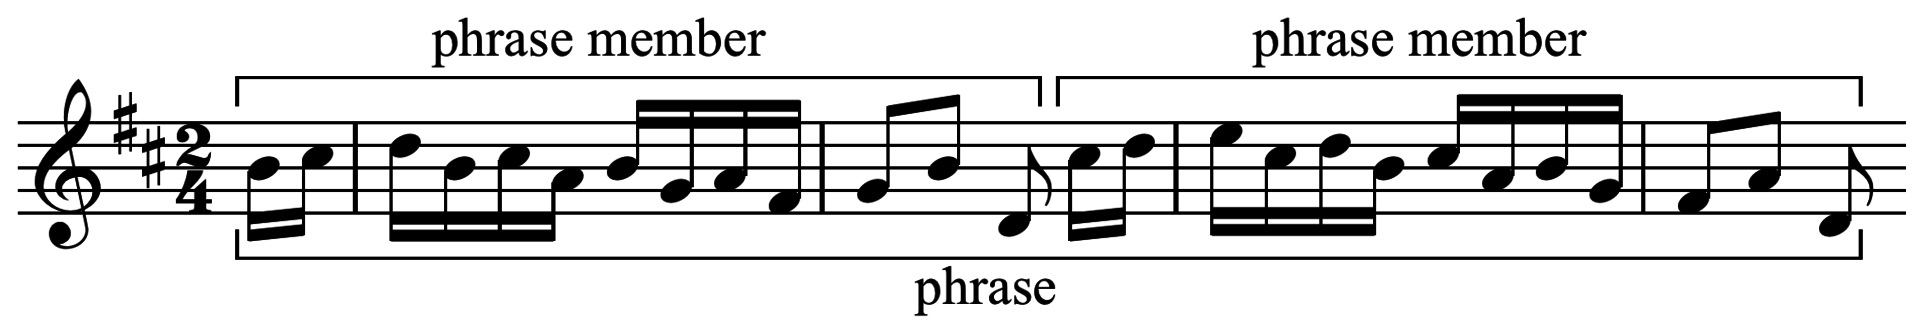
\includegraphics[width=\textwidth]{diagrams/Haydn}
\caption{Example of balanced phrase pair from  Haydn's Trio no. 1 in G Major}
\label{haydn}
\end{figure}

The clarity of the structure in music of this era means that musicologists often depend on this style to describe phrasing. This is the case in \cite{Bod_probabilisticgrammars}, where Mozart's famous G Minor Symphony is used for this purpose.

%other styles are not so simple. Music from the romantic era is characterised by long flowing phrases that are much more ambiguous.


%Nevertheless, while there is always some ambiguity, the majority of interpretations of phrase start and end points will be relatively uncontroversial.

\section{The Essen Folksong Collection}
\label{essensec}

While music from the classical era is used to describe phrasing to the reader, the actual examples that make up the corpus used for experiment come from the Essen Folksong Collection. This is a large corpus of European folksongs notated using the Essen Associative Code (ESAC). This provides a way of notating music using standard characters, which is therefore easy for computers to store and process. For a detailed description of how this notation works readers should see \cite{Bod_probabilisticgrammars}.

The Collection itself includes 6,251 folk melodies collected under the supervision of Helmut Schaffrath at The University of Essen \cite{essen}. Unlike standard Western musical notation, these melodies have phrasing stored along with the other melodic data. The fact that this data is encoded on such a large corpus gives the opportunity to train and test phrase prediction algorithms. Along with standard practice on the treatment of corpora in NLP, the Essen collection is divided randomly into training and test sets of ratio 5,251:1,000 respectively.  

For the purpose of testing these algorithms, it is necessary to have a system of scoring any generated solution. To do this, a methodology was borrowed from the field of NLP, as proposed in \cite{nlp-score}. This uses the twin notions of \emph{precision} and \emph{recall} defined as:
$$precision = \frac{\#\ correct\ phrases\ in\ P}{\#\ phrases\ in\ P} $$
and
$$recall = \frac{\#\ correct\ phrases\ in\ P}{\#\ phrases\ in\ T} $$
where $P$ is a proposed parse and $T$ is the test set parse from the corpus. Another concept from the field of NLP is used to combine these - that of the F-score. This is given in \cite{manning} as

$$ F\-score = \frac{2 \cdot precision \cdot recall}{precision+recall}. $$

Now that there is a corpus, complete with training and test sets, and a scoring algorithm, it is possible to unleash machine learning techniques devised for NLP on this problem.

\section{Parsing Techniques}

The paper provides results from 3 parsing techniques. The first and least successful of these is the Treebank grammar technique first proposed in \cite{Bod93}. This is an extremely simple context-free technique that stores all structures in the training set and derives a probability based on the frequency of these structures within the training set.

This technique yields a precision of 68.7\%, a recall of 3.4\%, and an F-score of 6.5\% according to the definitions of these measures set out in \ref{essensec}.

The relative nature of these scores is explained by the conservative nature of this parsing technique. The grammar will only output a phrase when a string is provided that exactly matches a phrase in the training set. This means that of those phrases predicted by the parse a high proportion are indeed phrases (68.7\%). But, many phrases that do exist are ignored, yielding a very low score for recall and therefore a low F-score. The precision score would be higher if some contextual features where used in parsing, so that, for example, a common short phrase from the test set would not be predicted in a piece that otherwise has much longer phrases. The recall would be higher if there was some mechanism for predicting phrases that do not exactly exist within the test set.

The next proposed technique, a Markov grammar, addresses some of the conservativity of the Treebank method. This method is applied to NLP in \cite{Seneff1992}. This creates Markov chains at the note level in order to predict the likeliness of a phrase ending given the previous $n$ notes, where $n$ is the order of Markov process. In this case a third-order Markov process was used and produced a  precision of 63.1\%, a recall of 80.2\%, and an F-score of 70.6\%. While the precision in this case is slightly lower than that of the Treebank technique, as would be expected with a more permissive system, the recall is very much higher.

The third technique can be thought of as an extension to the Markov grammar described previously. This uses the Data-Oriented Parsing (DOP) technique to take into account a global context. This context allows factors such as average phrase length in the piece being parsed to be taken into account. As expected, this extra information improves all measured scores. The DOP-Markov parser obtained a precision of 76.6\%, a recall of 85.9\%, and an F-score of 81.0\%. 

Table \ref{resulttab} shows all of these results in full. The results can be summarised by comparing how much information these parsers take into account from their training. The Treebank only operates at the object level and therefore only remembers familiar objects from the training set. The Markov technique takes into account probabilistically the relation between notes, or sub-object elements, and therefore gives better results, although some precision is sacrificed as this yields a less conservative grammar. The final and most successful technique adds to this a global context. It is demonstrated in these cases, therefore, that the more probabilistic data gathered from the training set, the more accurate the phrase predictions will be.

\begin{table}
\centering
\begin{tabular}{ |c|c|c|c| } 
 \hline
 Parsing technique & precision & recall & F-score \\ 
 \hline
 Treebank & 68.7\% & 3.4\% & 6.5\% \\ 
 Markov Grammar & 63.1\% & 80.2\% & 70.6\% \\ 
 Markov + DOP & 76.6\% & 85.9\% & 81.0\% \\ 

 \hline
\end{tabular}
\caption{Table showing full results from the parsing experiments. The Markov and DOP technique was the most successful.}
\label{resulttab}
\end{table}

\section{Other Parsing Techniques}

The paper \cite{Bod_probabilisticgrammars} also includes a discussion of other parsing techniques. It describes most, if not all, of these as ``non-probabilistic''. Bod claims much of these techniques lack the formalism required to generate a parser. For example, depending on notions such as the musical cadence without definition is challenging. While such a device might be obvious to an experienced listener, subtlety in deployment of such techniques is typically seen as a virtue. This makes spotting such features a non-trivial task.

Other non-memory based methods of phrase prediction are discussed as borrowed from classical musical analysis, such as the use of melodic arches or pitch jumps. However, as seen in other fields of artificial intelligence, it seems unlikely that these bespoke methods of parsing will yield results comparable in quality to those of memory-based machine learning techniques.

\section{Critical Review}

The paper was generally extremely interesting and justifies its claim of successfully applying NLP parsing techniques to musical examples. This success is not altogether surprising, as similarities between natural languages and music have been part of discourse, at least artistic discourse, for likely as long as there has been either. The paper outlines important groundwork that was done to enable computational analysis of music, such as deriving an efficient, complete, and computable notation; gathering a suitably large corpus; and applying appropriate machine learning algorithms.

However, the claim made in the paper that previous attempts are entirely non-probabilistic does not hold up to very close scrutiny. A handwritten formal grammar for parsing music derived from principles from the field of musical analysis would be described as ``non-probabilistic'' by \cite{Bod_probabilisticgrammars} if it did not distinguish between the likelihood of different parses. It could be argued instead that this simply treats all valid parses as equally probable. Indeed, within the parsing techniques there are degrees to which probabilities are taken into account - the Treebank technique simply takes into account frequency of a given phrase, where Markov techniques take into account more context. Drawing from the realm of NLP, an analogue might be that of n-gram models. When predicting the next word in a sentence using such a model, the lowest order technique would be to assume all words in a dictionary are equally likely to appear next (this is the sort of analysis a simple spell-checker will do), a more probabilistic approach would be to predict high frequency words, and beyond this use $n$ previous words to derive a probability of the next word. It does not seem appropriate to draw a hard distinction between probabilistic and non-probabilistic approaches as done in \cite{Bod_probabilisticgrammars}. The distinction between treating all syntactically correct phrases as equally likely or not seems no more important than the distinction between treating all sequences of phrases as equally likely or not. A more subtle approach would be to view parsers as being on a probabilistic spectrum.

%Phrases are deterministic or not?
Such an analysis would go more to the heart of what the true nature of probability is - the art of dealing with incomplete information in a  rigorous fashion. The obvious example when discussing such matters is a coin toss. This is given as the archetypal probabilistic system, but, if all information is known of the physical properties of the coin as well as the coin's initial velocity, it should be possible to accurately predict the result. Whether all such systems are deterministic is a matter that divides philosophers and scientists alike - Einstein, in response to the theories of quantum mechanics that he helped initiate famously claimed that ``God does not play dice with the universe''. Just as some may argue about the determinism of sub-atomic physics, it is possible to argue about the determinism of musical phrasing. Given a string of note pitches and durations, is it possible to predict deterministically what consensus will be within a musical community? Or perhaps there is some creative magic along the way either due either to quantum effects in our brains, or divine inspiration, depending on your outlook. With the given corpus this paper seems to answer the question fairly conclusively. The fact that very accurate phrasing predictions are yielded from the best parser shows that phrasing is strongly deterministic for this data set.

%Folk music is triv.
However,  different musical genres take different approaches to phrasing. The corpus selected is the European folksong style. Little analysis is given in \cite{Bod_probabilisticgrammars} as to whether the predictability of music of this genre is more pronounced than others. It seems very likely that this is the case. As discussed in \ref{phrases}, music of the Classical period typically has well defined, predictable phrasing. This is perhaps more true of folksong - which is known for its simplicity. While \cite{Bod_probabilisticgrammars} alternates in its discussion between these two genres, it does little to compare the predictability of phrasing of the two. Even more interesting would be the application of parsing techniques to different musics that prioritise less predictable phrasing, or even shun the concept of phrasing completely. An analogue from NLP would be the parsing of different natural languages. However, it seems more likely that success in the realm of music will be harder to achieve. Most, if not all, natural languages share concepts such as verbs, nouns, or adjectives. There is much less agreement as to what constitutes music and whether elements such as rhythm, tone or structure are essential. The clich\'ed example of this would be 4'33'' by John Cage which has none of these elements. It seems likely that the relative determinism of different genres of music varies. Pursuing this as a future avenue of enquiry appears as though it would be fruitful, although applying parsers to different genres would require the expensive effort of compiling and notating an appropriate corpus for each.

%Writing music probabilistically is uncreative and bad
The process of deriving and emphasising correct phrasing is generally seen within the Western Art music tradition as an act of creativity, with performance artists praised or criticised for how well they perform this task. Given the success of algorithmic approaches to phrase prediction, it seems natural to consider how well such algorithms and formal grammars might cope with what many would say is the ultimate creative task in music - composition. It is argued here that algorithmic composition using formal grammars can never be truly creative. While a parser could be used to generate an output that is matches another musical syntax, this syntax can only be learnt from human creativity. This learning can only take in up to 100\% of the grammar rules that make the style. However, human art does not stand still, and each composer will add or remove grammatical elements within their style. This could be simulated by allowing random fluctuations into the generation of musical grammars. However, this would simply leave the creative process to the curation of these grammars and their outputted artwork. 

\section{Conclusion}
The parallel between the analysis of language and music is a notable one, as both involve the difficult work of formalising what is very natural to most people. 

The paper reviewed shows the potential of using formal grammars trained on a large corpus to analyse music of the European folksong style. The successful application of NLP techniques is particularly promising as it provides evidence the field of music informatics can benefit from work done in this much more extensively researched area. There is interesting further work in determining whether these techniques could be applied to other musical genres. This report has included some discussion as to whether such techniques might be successful.

It has been argued here that grammars could well be useful in generating music of a certain style, but cannot do the creative work of making new art. All work generated using such techniques will either be entirely derivative of previous work, or be randomly deviant from such work and require other artistic curation.

\bibliography{bibliography}
\bibliographystyle{ieeetr}

\end{document}